\RequirePackage{luatex85}
\documentclass[border=1pt]{standalone}

\usepackage{tikz}
\usepackage{fixltx2e}
\usetikzlibrary{math, arrows, patterns, decorations.text}

\def\hexagonsize{0.5cm}
\pgfdeclarepatternformonly
	{hexagons}% name
	{\pgfpointorigin}% lower left
	{\pgfpoint{3*\hexagonsize}{0.866025*2*\hexagonsize}}%  upper right
	{\pgfpoint{3*\hexagonsize}{0.866025*2*\hexagonsize}}%  tile size
	{% shape description
	  \pgfsetlinewidth{0.4pt}
	  \pgftransformshift{\pgfpoint{0mm}{0.866025*\hexagonsize}}
	  \pgfpathmoveto{\pgfpoint{0mm}{0mm}}
	  \pgfpathlineto{\pgfpoint{0.5*\hexagonsize}{0mm}}
	  \pgfpathlineto{\pgfpoint{\hexagonsize}{-0.866025*\hexagonsize}}
	  \pgfpathlineto{\pgfpoint{2*\hexagonsize}{-0.866025*\hexagonsize}}
	  \pgfpathlineto{\pgfpoint{2.5*\hexagonsize}{0mm}}
	  \pgfpathlineto{\pgfpoint{3*\hexagonsize+0.2mm}{0mm}}
	  \pgfpathmoveto{\pgfpoint{0.5*\hexagonsize}{0mm}}
	  \pgfpathlineto{\pgfpoint{\hexagonsize}{0.866025*\hexagonsize}}
	  \pgfpathlineto{\pgfpoint{2*\hexagonsize}{0.866025*\hexagonsize}}
	  \pgfpathlineto{\pgfpoint{2.5*\hexagonsize}{0mm}}
	  \pgfusepath{stroke}
	}

\tikzstyle{distArrow} = [<<->>, shorten >=8pt, shorten <=8pt, thick, line width=4pt]
\tikzstyle{dist2Arrow} = [|<->|, thick, line width=4pt]
\tikzstyle{pointer} = [->, shorten >=8pt, shorten <=14pt, thick, line width=2pt]
\tikzstyle{textStyle} = [fill=white!90!black, font=\Huge]
\tikzstyle{textLine} = [pos=5.5,sloped,above, font=\Huge, fill=white]
\tikzstyle{lineStyle} = [line width=4pt,dotted]
\tikzstyle{line2Style} = [black!50!white, line width=4pt,dashed]

%%%%%%%%%%%%%%%%%%%%%%%%%%%%%%%%%%%%%%%%%%%%%%%%%%%%%%%%%%%%%%%%%%%%%%%%%%%%%%%%
%%%%%%%%%%%%%%%%%%%%                 colours                %%%%%%%%%%%%%%%%%%%% 
%%%%%%%%%%%%%%%%%%%%%%%%%%%%%%%%%%%%%%%%%%%%%%%%%%%%%%%%%%%%%%%%%%%%%%%%%%%%%%%%

\definecolor{tugreen}{RGB}{128, 186, 38}
\definecolor{tucitron}{RGB}{249, 219, 0}



%%%%%%%%%%%%%%%%%%%%%%%%%%%%%%%%%%%%%%%%%%%%%%%%%%%%%%%%%%%%%%%%%%%%%%%%%%%%%%%%
%%%%%%%%%%%%%%%%%%%%                 Boxes                  %%%%%%%%%%%%%%%%%%%% 
%%%%%%%%%%%%%%%%%%%%%%%%%%%%%%%%%%%%%%%%%%%%%%%%%%%%%%%%%%%%%%%%%%%%%%%%%%%%%%%%
\tikzstyle{normalBox} = [shape=rectangle, draw=black, text=black, thick, 	
	align=center, fill=white]

\tikzstyle{roundBox} = [shape=circle, draw=black, text=black, thick, 	
	align=center, fill=white]

\tikzstyle{alternBox} = [shape=rectangle, text=white, thick, align=center, 
	fill=black, rounded corners]


%%%%%%%%%%%%%%%%%%%%%%%%%%%%%%%%%%%%%%%%%%%%%%%%%%%%%%%%%%%%%%%%%%%%%%%%%%%%%%%%
%%%%%%%%%%%%%%%%%%%%                 Arrows                 %%%%%%%%%%%%%%%%%%%% 
%%%%%%%%%%%%%%%%%%%%%%%%%%%%%%%%%%%%%%%%%%%%%%%%%%%%%%%%%%%%%%%%%%%%%%%%%%%%%%%%

\tikzstyle{normalArrow} = [thick,->,>=stealth, draw=black]

\usepackage[utf8]{inputenc}
\usepackage[T1]{fontenc}
\usepackage[sfdefault]{FiraSans}
 

\begin{document}
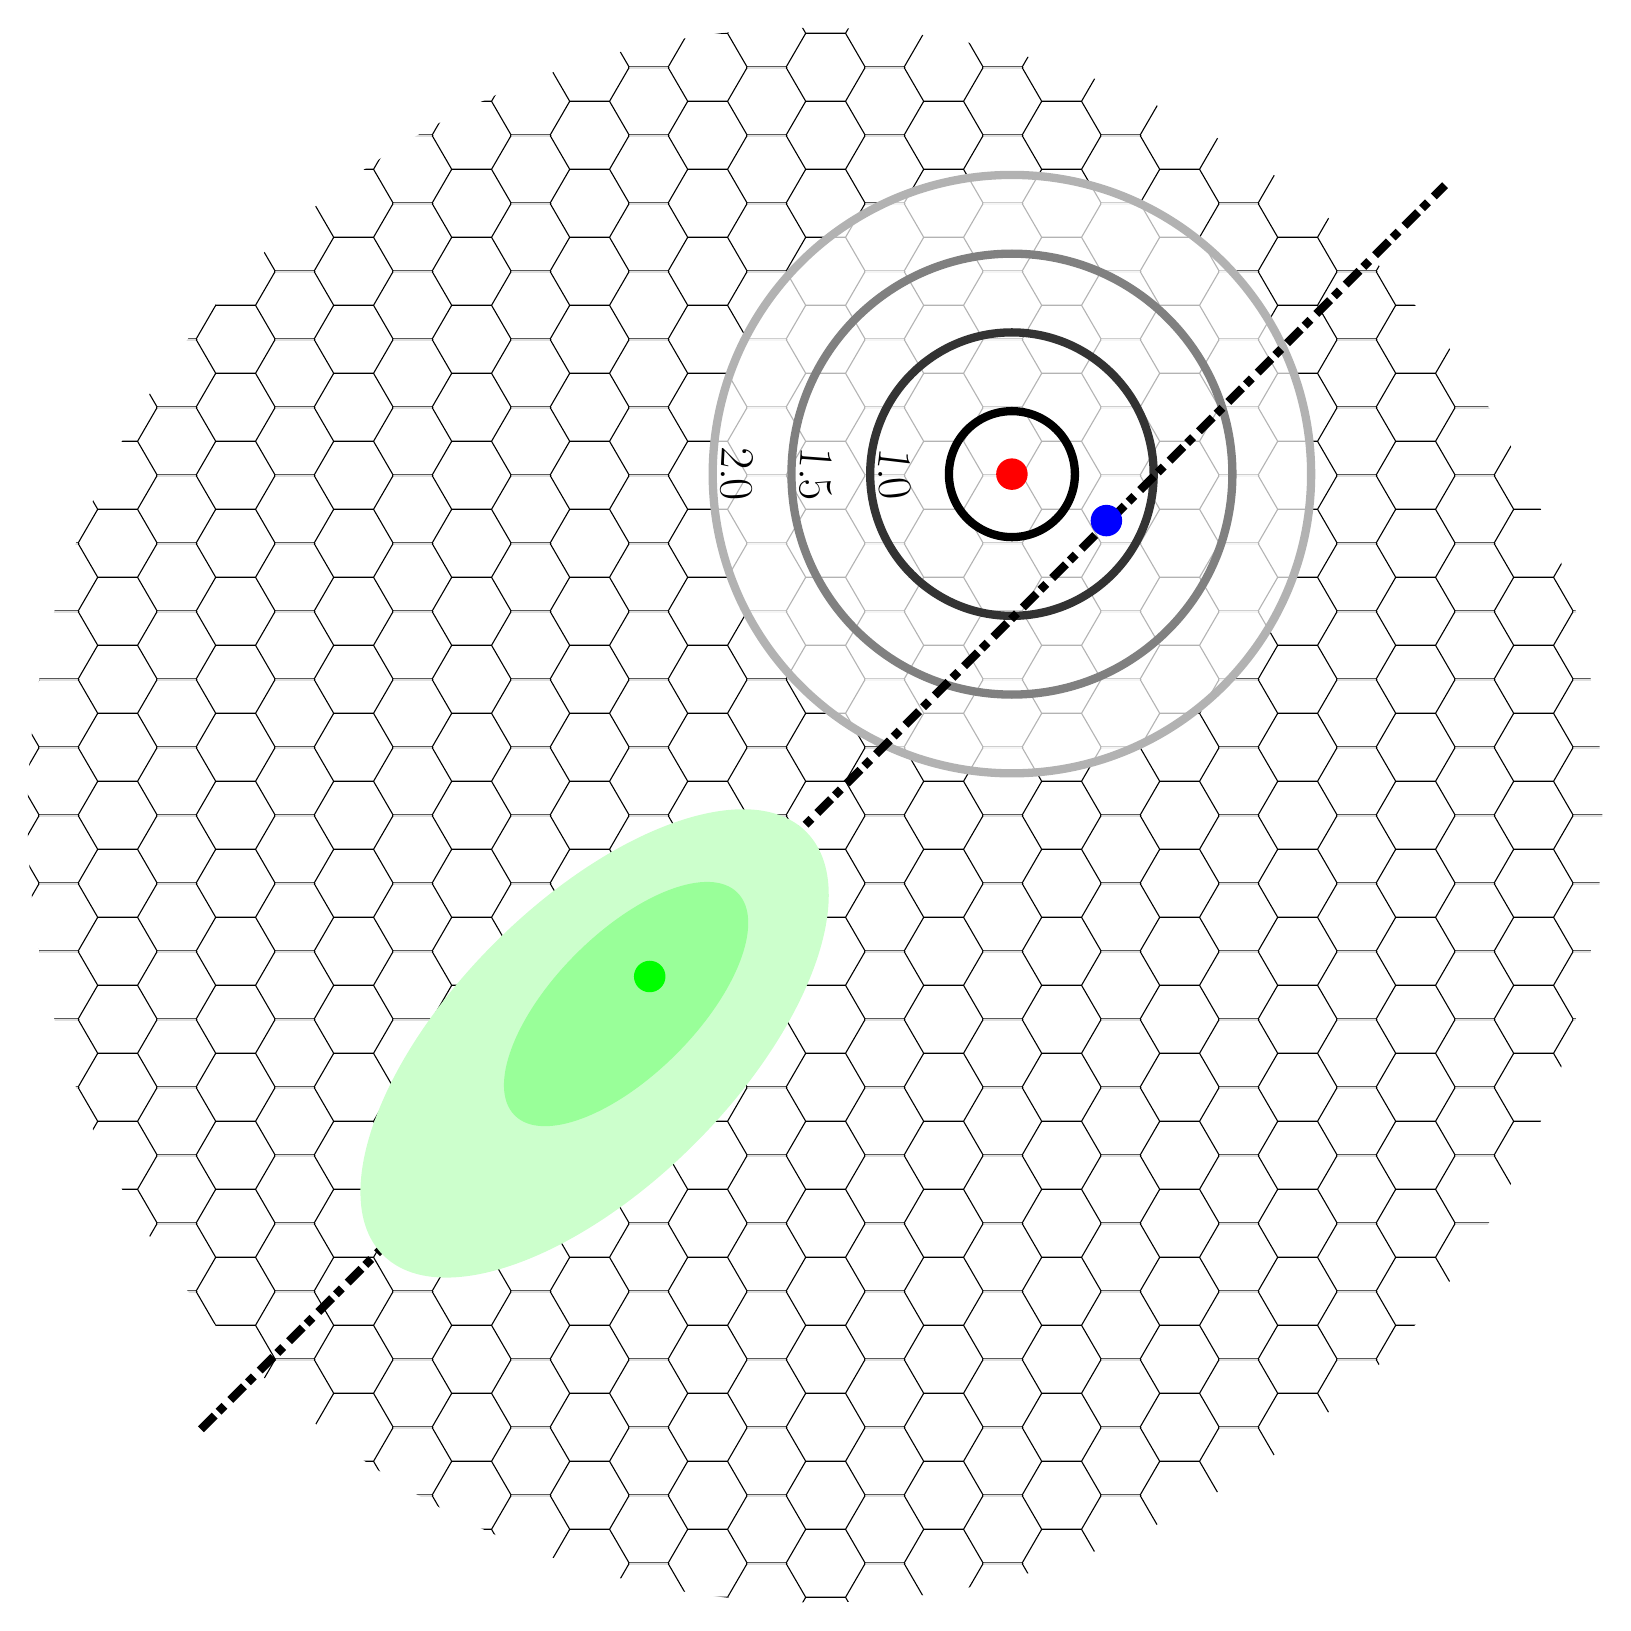
\begin{tikzpicture}
  %zeichnet hexagonales Rundes Grid
  \fill[pattern=hexagons] (0,0) circle (10cm);
 
  %Region expected source

  
  \draw[fill=white, opacity=0.7] (2.5 , 4.33) 	circle [radius=3.8];
	\LARGE
  \draw[black!30!white, postaction={decorate}, decoration={text along path, text={2.0},text align=center, raise=0.4ex}, line width=3pt](2.5 , 4.33) 	circle [radius=3.8];
  \draw[black!50!white, postaction={decorate}, decoration={text along path, text={1.5},text align=center, raise=0.4ex}, line width=3pt](2.5 , 4.33) 	circle [radius=2.8];
  \draw[black!80!white, postaction={decorate}, decoration={text along path, text={1.0},text align=center, raise=0.4ex}, line width=3pt](2.5 , 4.33) 	circle [radius=1.8];
  \draw[black!100!white, line width=3pt](2.5 , 4.33) 	circle [radius=0.8];

  % Non Noff positions
  \fill[fill=red]  	(2.5 , 4.33)	circle [radius=0.2];

  \draw[line width=3pt, dash pattern={on 7pt off 2pt on 3pt off 3pt}] (-7.8,-7.8) -- (8,8);
  \fill[fill=blue] (3.7, 3.74) circle [radius=0.2];

  % Con core of image 
  \fill[fill=green!20] (-2.8,-2.9) circle [x radius=38mm, y radius=18mm, rotate=45];
  \fill[fill=green!40] (-2.4,-2.4) circle [x radius=20mm, y radius=9mm, rotate=45];
  \fill[fill=green] (-2.1, -2.05) circle [radius=0.2];

\end{tikzpicture}
\end{document}
